%Version en ligne
\documentclass[12pt,a4paper]{report}
%Version imprimable
%\documentclass[12pt,a4paper,twoside,openright]{report}
% ************************
% * fichier de pr�ambule *
% ************************

% ***** extensions *****
\usepackage[T1]{fontenc}        % Caract�res accentu�s et c�sure
\usepackage[utf8x]{inputenc}    % Choix de l'encodage
\usepackage{graphicx}           % Paquage pour l'insertion d'images
\usepackage{wrapfig}            % Figures flottantes
\usepackage[french]{babel}      % Support Fran�ais
\usepackage{eurosym}            % Signe � qui s'adapte en fonction de la police
\usepackage{fancyhdr}           % En-t�te de pages personalis�s
\usepackage{color}              % Un peu de couleurs
\usepackage{array}              % Faire des beaux tableaux
% Liens cliquables dans le document
\usepackage[colorlinks=true,linkcolor=black,urlcolor=blue,%
pdftitle={Workshop},pdfauthor={GConfs}]{hyperref}
\usepackage{amsmath}            % Formules mat�matiques
\usepackage{listings}           % Mise en forme de code source

% Changement des polices du document
\usepackage{palatino}
\usepackage[sc]{mathpazo}
\linespread{1.05}

% ***** c�sures particuli�res *****

\hyphenation{}

% ***** filigrane *****
\newcommand{\makefiligrane}
{
   \usepackage{eso-pic,rotating}
   \AddToShipoutPicture{%
   \unitlength 1cm
   \put(11,15){%
   \begin{rotate}{45}
   \makebox(0,0){\color{lightgray}\scalebox{3.5}{\Huge BROUILLON}}
   \end{rotate}}
   }
}

% ***** couleurs perso *****

\definecolor{lightgray}{RGB}{240,240,240}

\definecolor{vert}{RGB}{0,176,80}
\definecolor{verta}{RGB}{79,97,40}
\definecolor{vertb}{RGB}{195,214,155}
\definecolor{vertc}{RGB}{235,241,221}
\definecolor{bleua}{RGB}{31,73,125}
\definecolor{bleub}{RGB}{219,229,241}
\definecolor{rougea}{RGB}{192,80,77}
\definecolor{rougeb}{RGB}{242,220,219}

\definecolor{brown}{RGB}{128,0,0}
\definecolor{blue}{RGB}{0,0,255}
\definecolor{green}{RGB}{0,128,0}
\definecolor{seagreen}{RGB}{69,158,181}


% ***** commandes personnelles *****
\newcommand{\helpbox}[3][bleu]{\vspace{1em}\fcolorbox{#1a}{#1b}{\parbox{.92%
\linewidth}{\hspace{5pt}\textbf{#2~:} #3}}\vspace{0.75em}}
\newcommand{\warnbox}[3][rouge]{\vspace{1em}\fcolorbox{#1a}{#1b}{\parbox{.92%
\linewidth}{\hspace{5pt}\textbf{#2~:} #3}}\vspace{0.75em}}
\newcommand{\tp}{workshop}
\newcommand{\Tp}{Workshop}
\makeatletter
\renewcommand{\chapter}{\clearpage%
     \@startsection{chapter}{1}{-0.75em}{\baselineskip}%
     {0.5\baselineskip}{\LARGE\textbf}}
\makeatother
\renewcommand{\thechapter}{\Roman{chapter}}
\renewcommand{\thesection}{\arabic{section}}

% ***** en-t�tes et pieds de pages *****
\newcommand{\headfootparams}[1]{
    \pagestyle{fancyplain}
    \lhead[\emph{\nouppercase{\leftmark}}]{\emph{\textit{\Tp{} #1}}}
    \chead{} 
    \rhead[\emph{\textit{\Tp{} #1}}]{\emph{\nouppercase{\leftmark}}}
    \lfoot[]{\small{\textit{GConfs 2011}}}
    \rfoot[\small{\textit{GConfs 2011}}]{}
}

% ***** param�tre de la coloration syntaxique *****
\newcommand{\lstsetparams}[4]{
    \lstset{language=[#1]#2,basicstyle=\ttfamily\footnotesize,%
        stringstyle=\ttfamily\color{brown},commentstyle=\color{green},%
        %numberstyle=\footnotesize,stepnumber=1,numbersep=7pt,%
        backgroundcolor=\color{vertc},frame=single,tabsize=2,breaklines=true,%
        breakatwhitespace=false,%
        classoffset=0,% Mots cl�s non reconnus
        morekeywords={#3},keywordstyle=\color{blue},%
        classoffset=1,% Noms de classes
        morekeywords={#4},keywordstyle=\color{seagreen},%
        classoffset=0
    }
}
%\lstsetparams{varient}{lang}{blue_keywords}{seagreen_keywords}


% ***** for code listings *****
\lstsetparams{Sharp}{C}{}{Value,Convert,Exp,Cst}

% ***** workshop title (used as pages' head) *****
\newcommand{\workshoptitle}{Graphique} % FIXME

% ***** page heading and foot *****
\headfootparams{\workshoptitle}

% ***** to display a "BROUILLON" in all pages *****
%\makefiligrane

\newcommand{\cas}{\textsc{GRA}}
\newcommand{\npi}{\textsc{npi}}

\begin{document}

\title{
  \vspace{1cm}
  \textbf{\Huge{\Tp{} \workshoptitle}}\\
  %\vspace{1cm}
  %\includegraphics[scale=0.75]{images/logo.png}
}
\author{
  \Large{Raphaël \textit{Shugo} \textsc{Boissel} ({\ttfamily boisse\_r})}\\\\
}

\date{
  \vspace{1cm}
  % GConfs logo
  
\includegraphics[scale=0.5]{gconfs.png}\\
  \vspace{0.5cm}
  Vendredi 23 Novembre 2012
}
\maketitle
\newpage
\tableofcontents
\newpage

\chapter{Introduction}
L'objectif de ce workshop est la réalisation d'un petit jeu dans lequel nous
nous focaliserons principalement sur tout les problème de rendu graphique.
Le jeux qui vas être réalisé est un pseudo R-Type.

\section{Fonctionnement du workshop}
Le workshop est divisé en palier successif (du plus facile au plus difficile). Chaque palier est divisé en deux
parties \textbf{ LISEZ  BIEN LES DEUX PARTIES AVANT DE COMMENCER LE PALIER}. Une première partie
décrit les objectifs du palier, une deuxième partie donne des indications sur la façon de le réaliser.
Afin d'éviter que ce workshop se transforme en un gros copier-coller de code ce qui serait un
peu ennuyeux, seul les grandes lignes, les principales fonctions et les pièges à éviter vous seront
donnés le code et la structure du code est entièrement à votre charge !
 

\section{Le choix des armes}
Dans ce workshop vous êtes libre de choisir l'outil de votre choix, de
préférence celui que vous utiliserez dans votre projet (XNA, DirectX, OpenGL, ou d'autres). 
Cependant nous vous conseillons vivement de ne pas avoir les yeux plus gros
que le ventre et de choisir DirectX ou OpenGL  \textbf{UNIQUEMENT} si votre projet l'exige
ou si vous êtes déjà familier avec ce type d'outils.

\section{Les Wrappers DirectX et OpenGL}
Pour pouvoir utiliser OpenGL ou DirectX en C\# il faut utiliser des wrappers.
Les wrappers se présentent généralement sous la forme de bibliothèques
reprenant une à une les fonctions de la bibliothèque de base dans une version
accessible depuis C\#. Voici les wrappers que nous vous conseillons mais rien ne
vous empèche de choisir le votre:\\
\begin{itemize}
\item SlimDX pour DirectX
\item OpenTX pour OpenGL\\
\end{itemize}

\textbf{NOTE}: en fonction du wrapper que vous choisirez vous
constaterez quelques légères différences dans le nommage des
fonctions ou dans celui  les paramètres :
par exemple openTK utilise \verb+Gl.Begin+ et Tao \verb+glBegin+

\chapter{L'interface}
\section{Afficher une fenetre}
\subsection{objectifs}
\begin{figure}[!h]\centering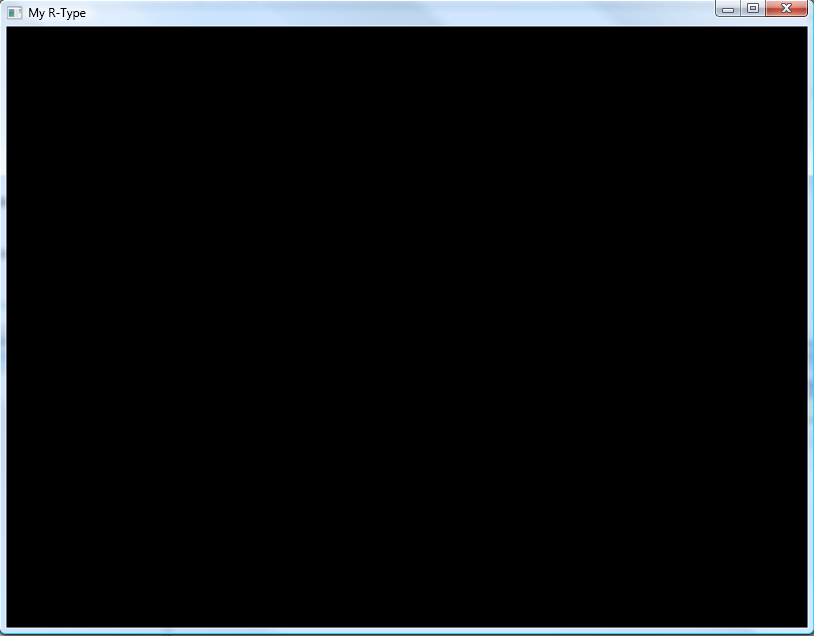
\includegraphics[width=7cm]{empty_windows.png}\end{figure}
Avant toute chose il faut ouvrir une fenetre. Si vous utilisez un outil comme XNA cela devrait-être un jeu d'enfant
en revanche si vous utilisez DirectX ou OpenGL la tache devrait être bien plus ardue. Ne négligez pas cette
étape un espace d'affichage mal configuré est souvent la cause de beaucoup de bugs et/ou lenteur
dans un jeu vidéo.

\subsection{conseils}
\begin{itemize}
\item \textbf{XNA}: Rien à faire tout est déjà prêt pour vous, passez à l'étape suivante.
\item\textbf{OpenTK}: créez une GameWindow n'utilisez pas de GLControl. (Les exemples d'openTK vous montreront comment créer une fenêtre basique à partir de gameWindow).
\item \textbf{SlimDX}:  \href{http://slimdx.org/tutorials/DeviceCreation.php}{Ouvrir une fenêtre avec slimSX}
\end{itemize}
\newpage

%---------------------------------------------------------------------------------------------------------------
\section{Dessiner un arriere plan}
\subsection{objectifs}
\begin{figure}[!h]\centering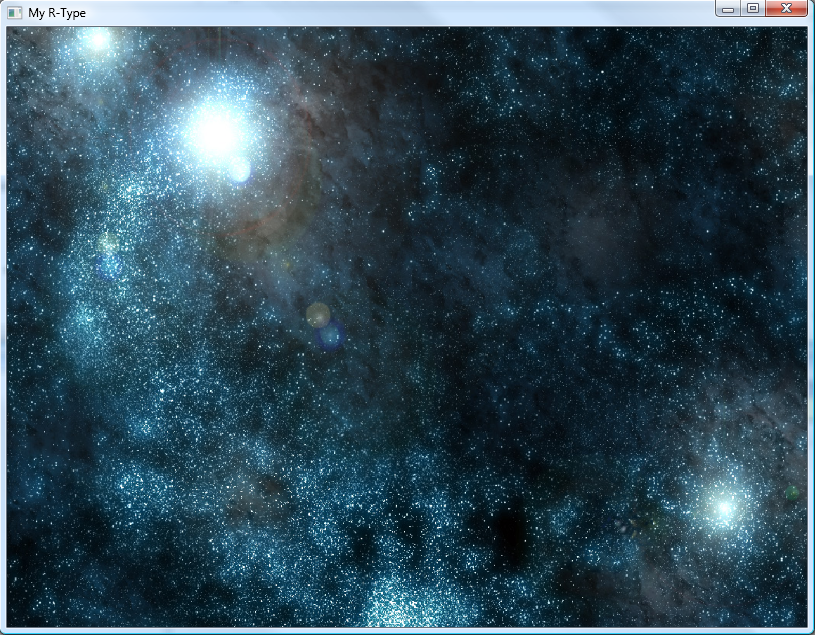
\includegraphics[width=7cm]{background_window.png}\end{figure}
Dans cette étape il "suffit" d'afficher un sprite qui occupe l'intégralité de l'arrière-plan. Profitez de cette étape pour
vous familiariser avec les fonctions de chargement d'image d'image ainsi qu'avec les fonctions de dessin.
La gestion de l'ordre de dessin ou de la transparence n'est absolument pas nécessaire ici.
\subsection{conseils}
\begin{itemize}
\item \textbf{XNA}: Utilisez la méthode  \href{http://msdn.microsoft.com/en-us/library/ff433986.aspx}{SpriteBatch.Draw} pour dessiner un sprite et utilisez
le \href{http://msdn.microsoft.com/en-us/library/bb197848.aspx}{ContentManager} pour charger l'image à afficher.
\item\textbf{OpenGL et DirectX}: Dessiner un sprite avec OpenGL ou DirectX reviens en fait à dessiner un polygone sur l'écran sans lui faire subir de transformation 3D et en lui appliquant une texture.
\item\textbf{OpenTK}: commencez par l'excédent  \href{http://nehe.gamedev.net/tutorial/your_first_polygon/13002/}{tutoriel de NeHe sur le dessin des polygonnes avec OpenGL} puis celui sur \href{http://www.opentk.com/doc/graphics/textures/loading}{le chargement de texture avec OpenTK}.
\item \textbf{SlimDX}: Lisez la \href{http://slimdx.org/tutorials/SimpleTriangle.php}{page sur le dessin de triangle avec slimDX} puis
regardez du côté des exemples fournis avec le \href{http://www.microsoft.com/en-us/download/details.aspx?id=6812}{SDK DirectX}.
\item \textbf{DirectX}: Regardez aussi du côté de D3DX avec \href{http://msdn.microsoft.com/en-us/library/bb172797(v=vs.85).aspx}{D3DXCreateSprite}.
\end{itemize}
\newpage

%---------------------------------------------------------------------------------------------------------------
\section{Dessiner des sprites}
\subsection{objectifs}
\begin{figure}[!h]\centering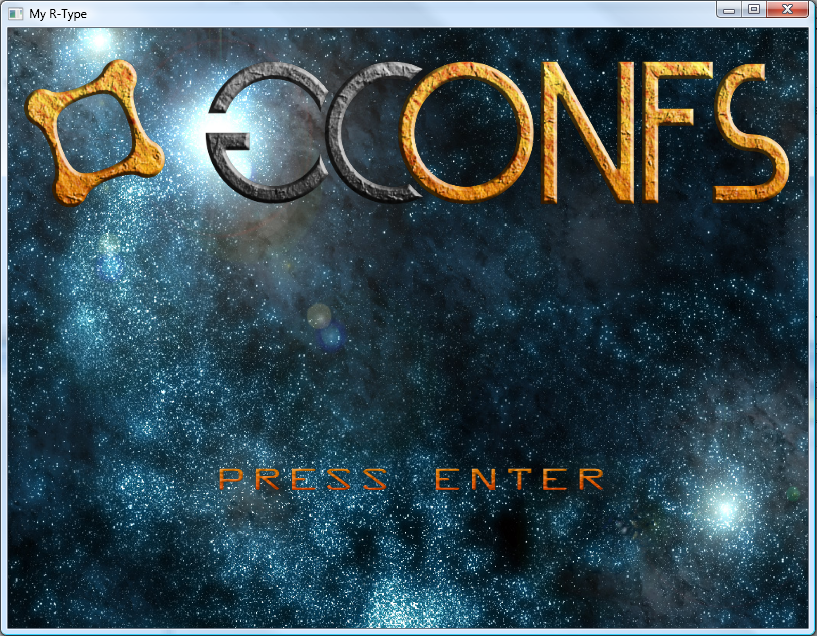
\includegraphics[width=7cm]{menu_window.png}\end{figure}
\begin{figure}[!h]\centering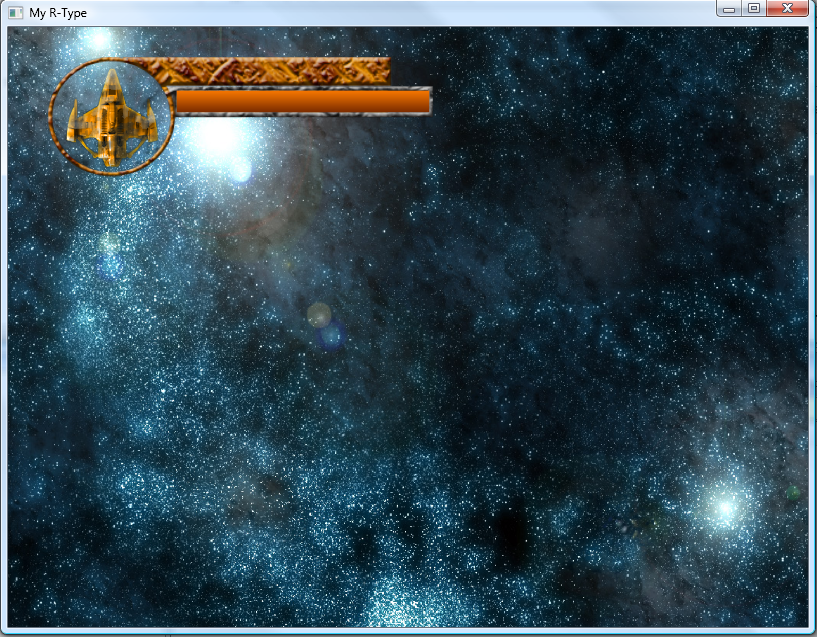
\includegraphics[width=7cm]{interface_window.png}\end{figure}
C'est ici que les choses sérieuses commencent ! Nous allons maintenant dessiner l'interface de notre jeu.
Une fois de plus pour ceux qui ont chosi XNA cela devrait être aussi facile que de dessiner l'arrière-plan.
Pour ceux qui ont choisi DirectX ou OpenGL cela ce corse. Il va falloir mettre en place du blending. Il s'agit de la
dernière étape 2D de ce workshop avant de passer à la 3D donc profitez bien de
cette étape pour finaliser toute votre interface afin que cela ne vous handicape pas plus tard.

\subsection{conseils}
\begin{itemize}
\item \textbf{XNA}: Rien de bien différent comparé à l'étape précédente, cette étape ne devrait pas poser de problème.
\item \textbf{OpenGL et DirectX}: Il va vous falloir configurer le blending(mélange de couleur) afin de pouvoir gérer la transparence. Le blending
doit être configuré de sorte que: $source = source * source.alpha$ $destination = destination * (1.0 - source.alpha)$.
\item \textbf{OpenGL}: utilisez \href{http://nehe.gamedev.net/tutorial/blending/16001/}{glBlendFunc} pour configurer le blending avec openGL.
\item \textbf{DirectX}: quand à directX vous trouverez les fonctions pour configurer le Blending sur \href{http://msdn.microsoft.com/en-us/library/windows/desktop/bb206241(v=vs.85).aspx}{MSDN}.
\end{itemize}
\newpage

%---------------------------------------------------------------------------------------------------------------
\section{Un peu de logique ...}
\subsection{objectifs}
Pas de programmation graphique ici. Le but de cette étape et de donner vie à notre interface:
implémentez la barre de vie, le passage de l'écran de démarrage à l'écran de jeu ...
\subsection{conseils}
\begin{itemize}
\item mettez en application ce que vous avez appris pendant le workshop BDSP (si vous y étiez).
\end{itemize}
\newpage

%---------------------------------------------------------------------------------------------------------------
\chapter{Et maintenant de la 3D}
En ce qui concerne la 3D et contrairement à la 2D nous ne recommandons pas l'utilisation de XNA.
En effet, ce dernier peut se révéler plus frustrant qu'autre chose lorsqu'il s'agit de faire de la 3D.
Cependant, sachez que rien ne vous empêche d'utiliser XNA malgré tout.

\section{Mon vaisseau c'est un cube !}
\subsection{objectifs}
\begin{figure}[!h]\centering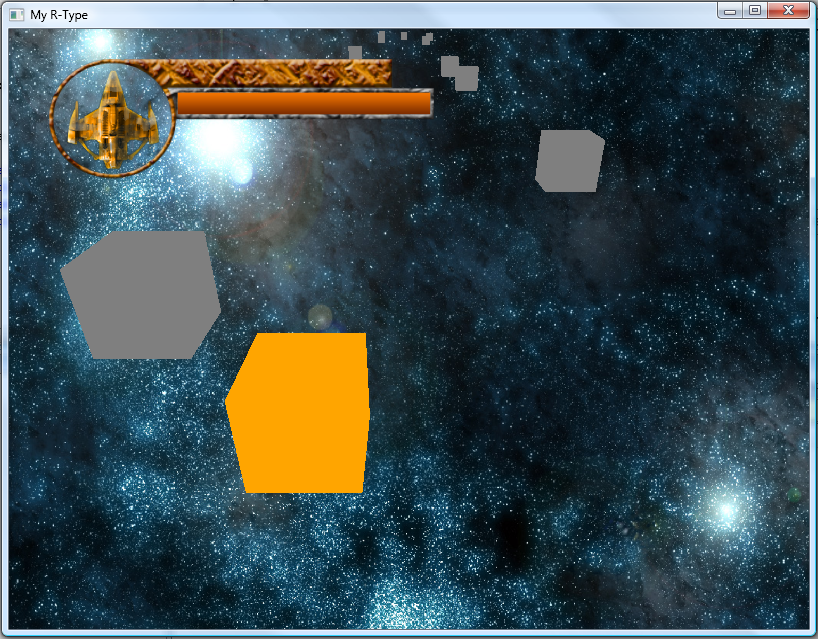
\includegraphics[width=7cm]{cube_window.png}\end{figure}
Cela peux sembler simple, voire simpliste, mais détrompez-vous, passer ce palier est probablement l'une des
étapes les moins aises du workshop. Pour pouvoir afficher ces cubes, vous allez devoir :
\begin{itemize}
\item Configurer et utiliser le Z-Buffer.
\item Créer vos matrices de transformation ("lookAt" pour la caméra et "translate" pour les objets).
\item Dessiner des polygones.
\end{itemize}

\subsection{conseils}
\begin{itemize}
\item \textbf{XNA}: Créez vos polygones en faisant un tableau de \href{http://msdn.microsoft.com/en-us/library/microsoft.xna.framework.graphics.vertexpositioncolor.aspx}{VertexPositionColor} et dessinez les avec 
\href{http://msdn.microsoft.com/en-us/library/bb196411.aspx}{GraphicsDevice.DrawUserPrimitives}.
\item \textbf{OpenGL}: une fois de lisez \href{http://nehe.gamedev.net/tutorial/3d_shapes/10035/}{les articles de NeHe}
\item \textbf{DirectX}: Les exemples du SDK DirectX contiennent toutes les informations pour comprendre comment réaliser cette tache.
\end{itemize}
%---------------------------------------------------------------------------------------------------------------
\newpage
\section{Des particules}
\subsection{objectifs}
\begin{figure}[!h]\centering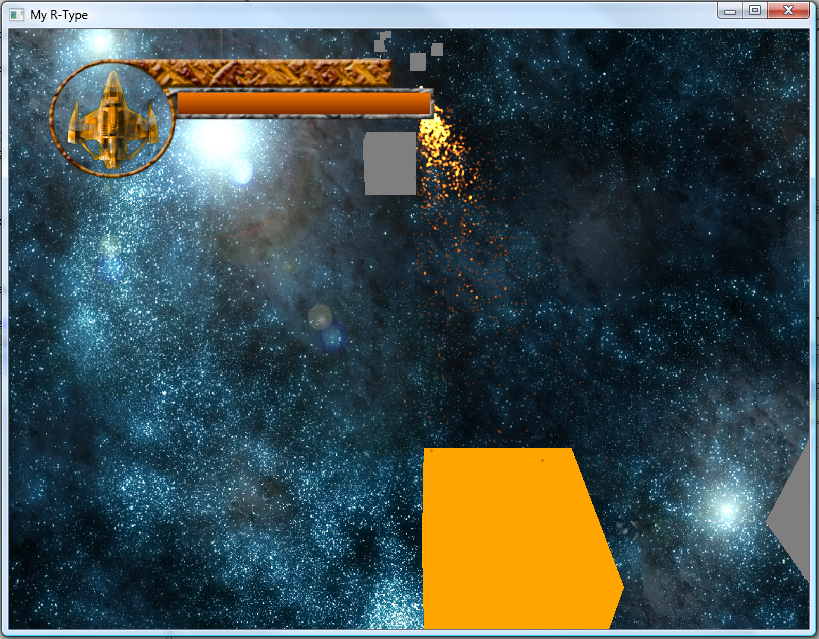
\includegraphics[width=7cm]{particles_window.png}\end{figure}
C'est bien tout ça, mais ça manque un peu d'action. Nous allons maintenant
faire en sorte que nos vaisseaux puissent tirer des projectiles.
Pour cela nous allons utiliser des particules. Cette étape n'est pas vraiment
indispensable pour la suite. Si vous la trouvez trop compliquée ou que vous
voulez vite passer à la suite, utilisez simplement une sphère ou tout autre objet de
votre choix afin de représenter les projectiles de votre vaisseau et ceux des ennemies.
\subsection{conseils}
Cette étape est optionnelle utilisez la technique avec laquelle vous vous sentez le plus à l'aise
les commandes ci-dessous ne sont que des suggestions. Cette étape n'est pas évidente à réaliser,
ne bloquez pas dessus et passez à la suite si vous ne voyez pas comment faire.
\begin{itemize}
\item \textbf{XNA et DirectX} calculez la position à l'écran (en 2D donc) de l'endroit ou vous souhaitez dessiner des particules (un point en 3D), puis dessinez vos particules sous forme de sprites.
\item \textbf{OpenGL} dessinez des points avec \verb+GL_POINTS+ dans votre fonction de dessins en lieu et place de \verb+GL_TRIANGLES+, puis faites les quelques ajustements nescessaires.
\end{itemize}
\newpage

%---------------------------------------------------------------------------------------------------------------
\section{Charger de vrai objets}
\subsection{objectifs}
\begin{figure}[!h]\centering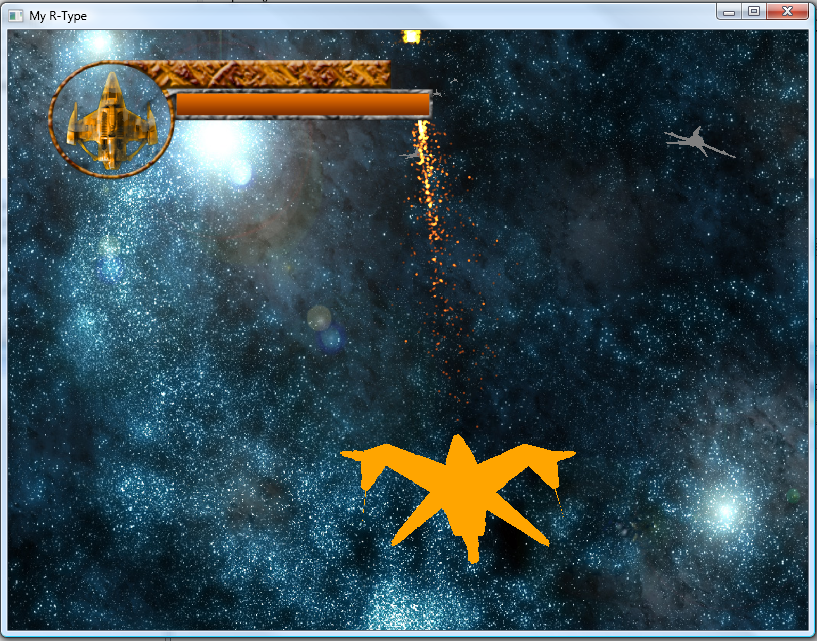
\includegraphics[width=7cm]{model_window.png}\end{figure}
C'est le moment de donner un côté un peu moins cubique à ce petit projet. Une fois de
plus remplacer les cubes par des objets sera une tache plus ou moins aisée selon vos choix. Et c'est sans nul doute
ceux qui ont choisi openGL qui auront le plus de pain sur la planche ici.
\subsection{conseils}
\begin{itemize}
\item \textbf{XNA} utilisez de nouveau le \href{http://msdn.microsoft.com/en-us/library/bb197848.aspx}{ContentManager}.
\item \textbf{DirectX} utilisez \href{http://msdn.microsoft.com/en-us/library/bb172890(v=vs.85).aspx}{les outils D3DX}.
\item \textbf{OpenGL} il va vous falloir charger votre fichier "à la main". Utilisez format wavefront qui est très simple à lire. Bon courage.
\end{itemize}

%---------------------------------------------------------------------------------------------------------------
\newpage
\section{Un peu de mouvement}
\subsection{objectifs}
Cette étape ne constient pas vraiment de phase graphique. L'objectif est ici de donner vie
à notre petit jeu :\\
\begin{itemize}
\item finalisez le déplacement de votre vaisseau et de celui de vos ennemies.
\item finalisez l'apparition des énemies.
\item gérez le score du joueur.
\item rendez ce programme fun !
\end{itemize}

\subsection{conseils}
Faites vous plaisir !
\newpage

%---------------------------------------------------------------------------------------------------------------
\chapter{Shaders}
Cette dernière partie est beaucoup plus difficile que les précédentes et nous
vous conseillons de vous y attaquer uniquement si vous vous sentez particulièrement à l'aise
en programmation et plus spécifiquement en programmation graphique.
\section{Lumière}
\subsection{objectifs}
\begin{figure}[!h]\centering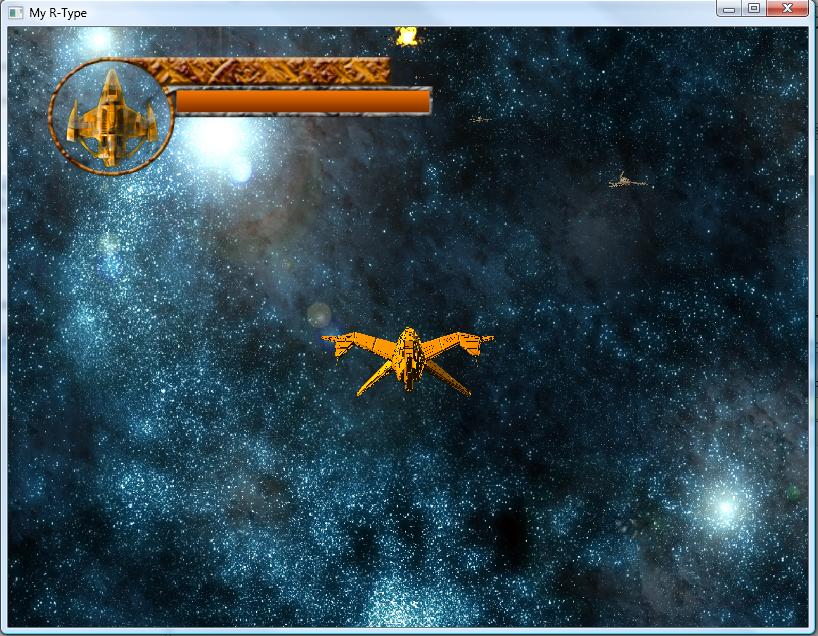
\includegraphics[width=7cm]{light_window.png}\end{figure}
Ici nous allons enfin passer aux choses sérieuses et nous allons utiliser des shaders. La première
étape de cette section consacrée au shaders consiste à implémenté illumination
de type Lambert (l'une des plus simples).
\newpage

%---------------------------------------------------------------------------------------------------------------
\section{Ombrage celluloide}
\subsection{objectifs}
"L'ombrage celluloïd a été inventé par des informaticiens pour pallier l'absence
de graphiste compétent dans certains studios de jeux vidéo" \footnote{phrase de Pannos
Baroudjan (Promo 2012) lors d'une de mes conversations avec lui, ma mémoire
étant ce qu'elle est il ce peux que les termes ne soient pas exactement ceux-ci, mais l'idée est la}.
Tout est dit !
\subsection{conseils}
\begin{itemize}
\item un obrage celluloïd est composé uniquement de quelques modiffication au modèle de Lambert.
\item pour gérer les contours pensez à étudier la valeur du produit scalaire de la normale d'un point avec
le vecteur donnant l'orientation de la caméra.
\end{itemize}
\newpage


%---------------------------------------------------------------------------------------------------------------
\chapter{Conclusion}
\begin{figure}[!h]\centering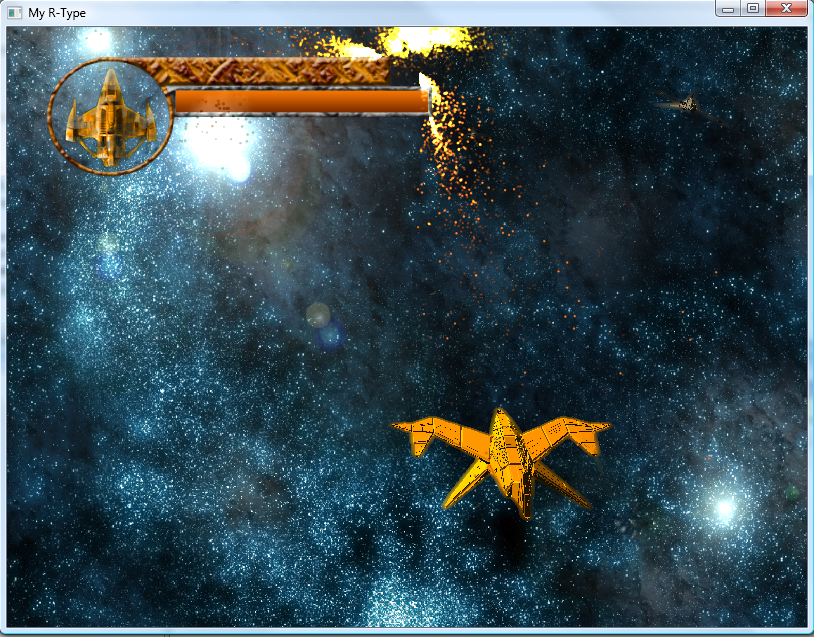
\includegraphics[width=7cm]{full_window.png}\end{figure}

Have fun !
 \end{document}